\chapter{The CMS GEM Project}
\label{chap:gem}

    In this chapter, we review the functioning and the mechanical design of GEM detectors, and present the performances obtained with GEM prototypes. We then state the problems that the actual CMS muon spectrometer will face after the LS1 and LS2 upgrades of the LHC, and motivate the proposition to install GEM detectors in the forward region of CMS instead of RPCs.

    \section{Physics Motivations}

        Why we need an upgrade and why the GEMs are good

    \section{Triple-GEM Detector Design}

        The following describes the detectors' layout and functioning for an installation in the CMS muon spectrometer.

        \subsection{Chambers Mechanical Design}

            GEMs \Cite{GEM_Technical_Proposal, GEM_Construction, GEM_Construction_and_Performance} are made out of a 50 \um{} thick kapton foil coated with a 5 \um{} copper layer on each side, that is chemically drilled to create a honeycomb pattern of holes, as represented in Figure \ref{fig:gas_electron_multiplier_detectors__construction}. The holes have a diameter of 70 \um{} on both ends and a diameter of 50 \um{} in the middle. They are separated by 140 \um{}. \\

            \begin{figure}[h!]
                \centering
                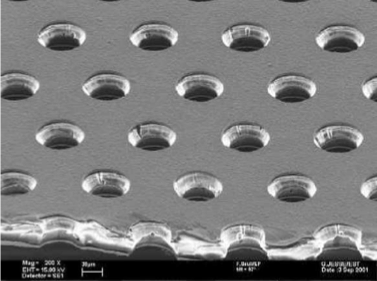
\includegraphics[height = 4cm]{gem/plate_view.png}
                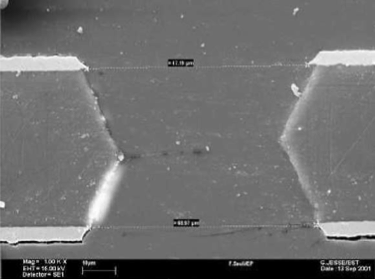
\includegraphics[height = 4cm]{gem/hole_view.png}
                \caption{Electron microscope view of the honeycomb pattern of holes in a GEM foil \Cite{GEM_Construction}.}
                \label{fig:gas_electron_multiplier_detectors__construction}
            \end{figure}    

            Three GEM foils are stretched and spaced by a few millimeters\footnote{The final design has not yet been chosen, leaving room for changes.} (1 to 3 mm) using a frame to form a Triple-GEM detector. A cathode plane is placed on one side and a series of anode strips (384 strips by 10$ ^\circ $ in $ \phi $) for the readout on the other. Figure \ref{fig:gas_electron_multiplier_detectors__structure} depicts the structure and the layers that compose a chamber. GEMs\footnote{In the rest of this work, \emph{GEM detectors} or simply \emph{GEMs} will refer to \emph{Triple-GEM detectors}.} have the same trapezoidal shape as CSCs as they would be installed in the endcaps. This means that even if the anodes are always spaced by 100 \um{}, the pitch between them (distance from middle to middle) is not constant, but varies between 600 \um{} on the narrow side and 1.2 mm on the long side. \\

            \begin{figure}[h!]
                \centering
                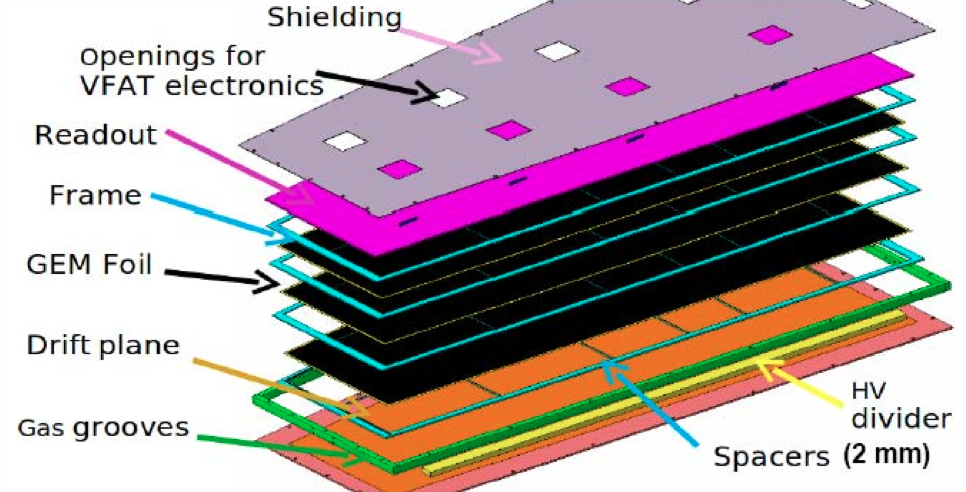
\includegraphics[width = 9cm]{gem/chamber_structure.png}
                \caption{Schematic view of the constitutive layers of a Triple-GEM detector \Cite{GEM_Test_in_Beam_1}.}
                \label{fig:gas_electron_multiplier_detectors__structure}
            \end{figure}        

            Each chamber covers 10$ ^\circ $ in $ \phi $ and is divided into 3 segments in $ \phi $ and 6, 8 or 10 segments in $ \eta $. This is done to
            \begin{enumerate}
                \item regroup a set of anodes into a single electronic readout chip; 
                \item increase the resolution in $ \eta $ as only the $ \phi $ coordinate is measured by the strips which leave a larger incertitude on the other coordinate;
                \item allow the detector to work even if a discharge occurs in one of the regions, requiring time to bring the voltage back up (the chamber's segmentation is not identical to the HV segmentation, but the argument remains valid).
            \end{enumerate}

            Once the detector is assembled, a gas mixture of Ar : CO$ _2 $ : CF$ _4 $ (45\% : 15\% : 40\%) is injected in the chamber. A voltage difference is applied between the two copper layers of each GEM foil to create a strong electric field inside the holes that act as multipliers. As represented on the left in Figure \ref{fig:gas_electron_multiplier_detectors__field_gain}, the field also channels the electrons towards the regions where they will be accelerated and create avalanches. Due to the geometry of the GEM foils, even a small voltage difference of the order of 400 V generates the intense fields (> kV cm$ ^{-1} $) required to initiate avalanches. Nevertheless, one amplification stage would not be enough to create detectable signals, justifying the presence of three layers. A graph representing the amplification according to the applied voltage and the number of layers is shown on the right in Figure \ref{fig:gas_electron_multiplier_detectors__field_gain}. This image depicts that increasing the number of GEM layers (SGEM stands for Singe-GEM, DGEM for Double-GEM, and TGEM for Triple-GEM) allows the system to be ran at lower voltage and achieve higher amplifications (continuous lines). The dotted lines illustrate the probability that a discharge occurs in the chambers. When using more GEM layers, the voltage range for which the probability is quasi null increases.

            \begin{figure}[h!]
                \centering
                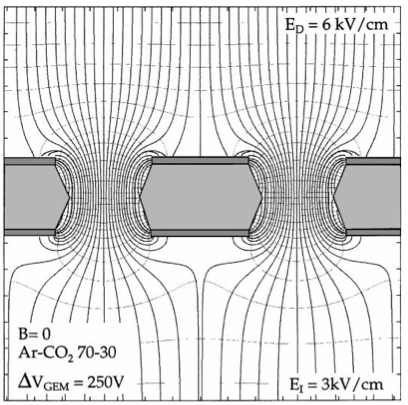
\includegraphics[height = 5cm]{gem/generated_efield.png}
                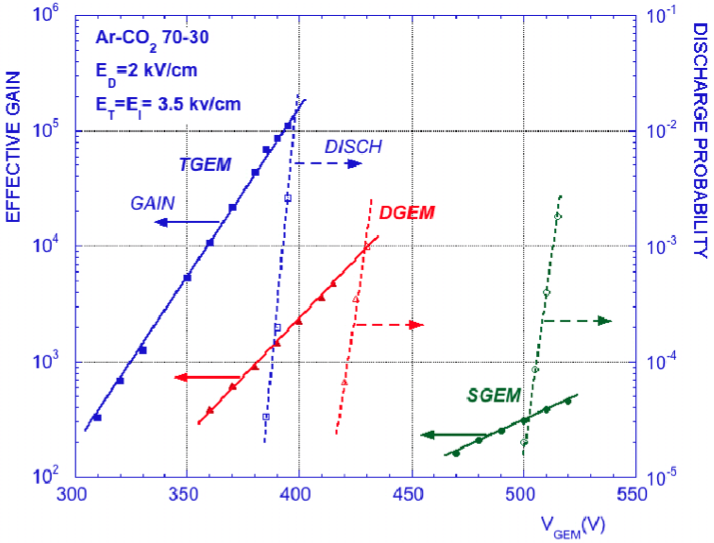
\includegraphics[height = 5cm]{gem/layers_gain.png}
                \caption{Representation of the electric field created inside the holes (left) \Cite{GEM_Electric_Field}; Gain for different numbers of GEM foils according to the applied voltage difference (right) \Cite{Thesis_Laura}.}
                \label{fig:gas_electron_multiplier_detectors__field_gain}
            \end{figure}    

            To improve the detection performances, two chambers are mounted back-to-back at each site, forming a \emph{super-chamber}.

        \subsection{Gas Electron Multiplier Principles}

            As reviewed in Section \ref{sec:gas_electron_multiplier_detectors__chamber_mechanical_design}, three foils are used in the GEM detectors' design, creating four gaps, as represented in Figure \ref{fig:gas_electron_multiplier_detectors__foils}.

            \begin{figure}[h!]
                \centering
                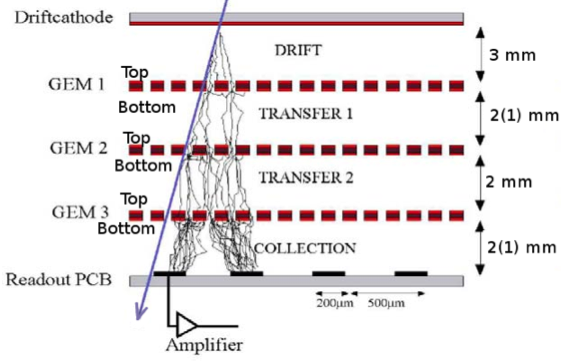
\includegraphics[width = 9cm]{gem/avalanche_in_foils.png}
                \caption{Signal amplification for a Triple-GEM detector \Cite{Thesis_Laura}.}
                \label{fig:gas_electron_multiplier_detectors__foils}
            \end{figure}

            Before describing the role of each gap, it is interesting to note that they can be seen as independent from one another, as the voltage difference applied on each side of the foils makes them look like electrode planes. Therefore, we can separate the function of GEMs into two parts: the electrons' multiplication that occurs between each gap, and the charges' drift that takes place inside a gap. Figure \ref{fig:gas_electron_multiplier_detectors__amplification} shows a simulation of the amplification performed by a Single-GEM. Electrons (orange) arrive from the right and are amplified inside the holes. The resulting electrons then continue their drift towards the left, scattering with the gas, while ions (red) are attracted by the previous foil's cathode.

            \begin{figure}[h!]
                \centering
                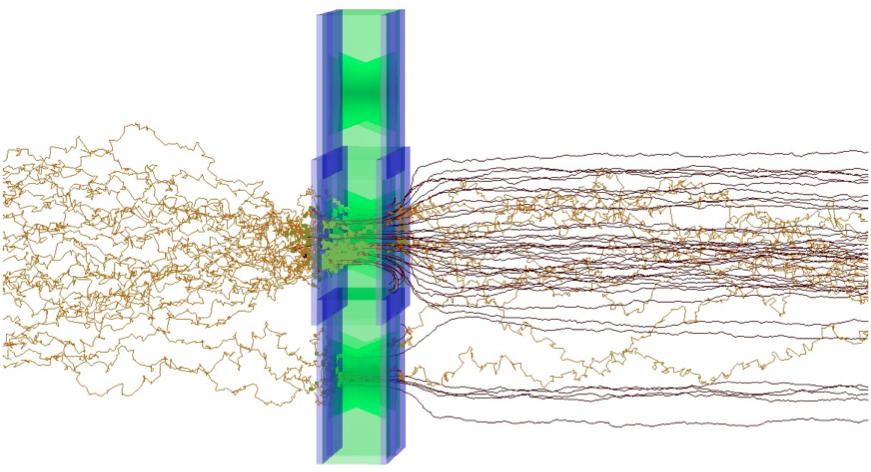
\includegraphics[width = 12cm]{gem/simulation_amplification.png}
                \caption{Simulation of the electrons' and ions' drift and multiplication for a Single-GEM foil \Cite{These_Geoffrey}.}
                \label{fig:gas_electron_multiplier_detectors__amplification}
            \end{figure}    

            Each gap plays a different role according to its width and to its order inside the chamber. The first gap is called the \emph{Drift gap}. It is where most of the detectable signals will originate from. It is larger than the other regions to increase the number of ionization clusters created by the particles. Electrons are then amplified by the first and second foil, and, respectively, enter the \emph{Transfer 1} and \emph{Transfer 2 gap}. Finally, after being amplified one last time, the electrons enter the \emph{Induction gap} where they will produce the readout signal. Due to the electrons' long drift distance in the last gap (1 or 2 mm), they are able to form a visible signal on the anodes, in opposition to the ions whose signal is a thousand times weaker as it is screened by the foils. \\

            We stated that only energy deposited in the Drift gap can be detected, which is not entirely true. If an energy loss occurs in the Transfer 1 gap and leaves behind a sufficient amount of energy, it can create a strong visible signal. With the same logic, multiple peaks can be observed in the Drift gap, corresponding to multiple energy losses. Table \ref{tab:gas_electron_multiplier_detectors__signal_timing} lists the arrival time ranges for the electrons originating from the different gaps. The mean drift speed of the electrons is of the order of 74.6 \um{} ns$ ^{-1} $. Figure \ref{fig:gas_electron_multiplier_detectors__raw_signal} represents the induced current on an anode inside a GEM detector filled with a gas mixture of Ar : CO$ _2 $ (70\% : 30\%) for a simulated muon of 1 \GeVc{} passing through the chamber perpendicularly to the readout plane. Each region defined with a red line corresponds to the signal created in a specific gap.

            \begin{table}[h!]
                \centering
                \begin{tabular}{l|l}
                    Gap & Timing \\ \hline
                    Induction & 0 - 14 ns \\
                    Transfer 2 & 14 - 42 ns \\
                    Transfer 1 & 42 - 56 ns \\
                    Drift & 56 - 98 ns 
                \end{tabular}
                \caption{Timing of the signals formed by the avalanches originating from the different gaps inside a Triple-GEM detector \Cite{GEM_Thierry_Pres}.}
                \label{tab:gas_electron_multiplier_detectors__signal_timing}
            \end{table}     

            \begin{figure}[h!]
                \centering
                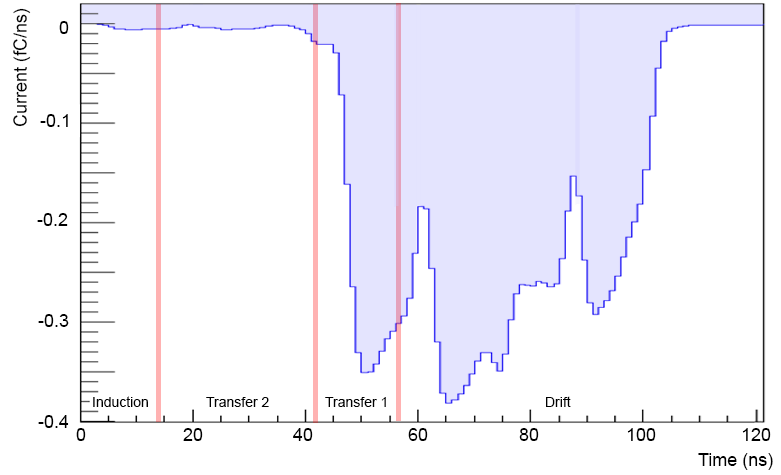
\includegraphics[width = 10cm]{gem/induced_e_signal.png}
                \caption{Simulation of the signal formed on the anodes by a single 1 GeV muon passing through the chamber perpendicularly to the readout plane \Cite{These_Geoffrey}.}
                \label{fig:gas_electron_multiplier_detectors__raw_signal}
            \end{figure}                

            The raw output signal is then shaped by the VFAT3 electronics which impulse response $ T(t) $, as defined in Section \ref{sec:muon_chambers__read_out_electronic}, is given by
            \begin{equation} 
                T(t) = \left( \frac{t}{\tau} \right)^2 \exp\left(- 2 \frac{t}{\tau} \right) \ ,
                \label{eq:gas_electron_multiplier_detectors__transfert_function}
            \end{equation}
            where $ \tau $ is the shaping time which can be programmed and take different values: 20, 50, 100, 250, or 500 ns. The shaping time has to be long enough to integrate the various peaks and always yield a well defined output signal function. 

        \subsection{GEM Foils Production}

            ???

    \section{Detector Performance}

        Small- and full-scale GEM prototypes have been tested using 150 \GeVc{} $ \pi / \mu $ beams \Cite{GEM_Construction_and_Performance, GEM_Test_in_Beam_1, GEM_Test_in_Beam_2, GEM_Test_in_Beam_3, GEM_Test_in_Beam_4}. Some of those results are presented in the following.

        \subsection{Detection Efficiency}

            Using test beam results, a maximal efficiency of 98\% is achieved for a single GEM detector. When using a super-chamber, the inefficiency of the system drops bellow 0.04\%.

        \subsection{Spatial Resolution}

            When the avalanche's charge hits only one strip, the spatial resolution is given by the pitch size of the strips divided by $ \sqrt{12} $, which is the variance of a uniform distribution. 
            \begin{equation} 
                \sigma_{\phi} = \frac{pitch}{\sqrt{12}} \approx 170 - 340 \, \mu m
            \end{equation}
            This theoretical value has been confirmed by the beam tests. \\

            Due to limitations in the amount of data that can be transfered from the detector to the storage units, it is possible that several strips will be regrouped into super-strips, or that the strips will be read in a binary mode (hit or not) instead of analogically (induced current). The granularity of the detectors is defined as the number of super-strips for each segment. It can be of 128, 64, 32, 16, or 8. The first one meaning that each strip acts like a super-strip, and the last one meaning that strips are regrouped in sets of 8. The lower the granularity, the higher the pitch, yielding a decrease of the spatial resolution.

        \subsection{Time Resolution}

            No algorithm to compute the resolution on BX assignment has yet been defined for the new VFAT3 electronics that will equip the CMS GEM detectors. However, a technique called \emph{Time Over Threshold} (TOT) is under study. Preliminary results show that this method is able to give the relative time at which a particle passed through the detector with a resolution of 4.44 ns \Cite{GEM_Thierry_Pres}. \\

            Figure \ref{fig:gas_electron_multiplier_detectors__tot} illustrates the TOT method by representing a shaped signal (blue) for the electronics, a clock pulse (red), and the defined threshold (black). Using the shaped signal, $ T_1 $ and $ T_2 $ are respectively define as the moment that the signal passes over, and below the defined threshold. The TOT, given by
            \begin{equation}
                TOT = T_{2} - T_{1} \ ,
            \end{equation}
            is measured with a clock running at a predefined frequency, yielding the number of clock cycles where the signal was above the threshold. The fact that the exact shape of the output signal (which only varies in amplitude) is known allows to run simulations that associate a specific arrival time to each value of the TOT. Those values are stored in a \emph{Look Up Table} (LUT). When a particle generates a signal, the number of clock cycles is measured and the arrival time is fetched in the LUT. If the shaping time of the electronics, the threshold value, or the clock speed are changed, a different LUT has to be generated. \\

            \begin{figure}[h!]
                \centering
                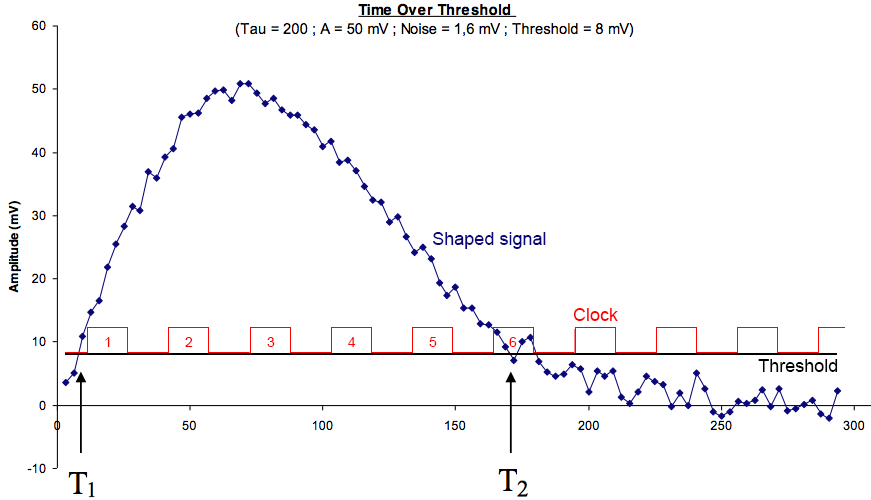
\includegraphics[width = 12.8cm]{gem/tot.png}
                \caption{Time Over Threshold (TOT) algorithm for Bunche Crossing (BX) assignment \Cite{GEM_Thierry_Pres}.}
                \label{fig:gas_electron_multiplier_detectors__tot}
            \end{figure}    

            The standard deviation of the Gaussian fit on the difference between the simulated arrival time and the value returned by the LUT, gives the time resolution of the detector.

        \subsection{Particle Rate Capability}

            Earlier work \Cite{GEM_Rates} demonstrated that GEMs can sustain rates up to 10 MHz cm$ ^{-2} $ before loosing detection efficiency. This is a strong argument in favor of the installation of GEMs in the high $ \eta $ regions of CMS where the rates are expected to be higher than 10 kHz cm$ ^{-2} $.   

    \section{Upgrade of the CMS Muon System}

        Events with high energy muons in their final state are a signature of many interesting processes such as the decay of the Brout-Englert-Higgs boson or possible new physics, like super-symmetry. Unfortunately, these events are rare and require a high detection efficiency and reconstruction capability. Even more so in the forward region of CMS where the tracks' projections in the transverse plane are shorter due to the high momentum of the muons, degrading the resolution on the reconstructed trajectory. \\

        As reviewed in Section \ref{sec:muon_chambers__disposition_of_the_detectors}, the muon system of CMS is not complete in the 1.6 < $ | \eta | $ < 2.4 region. Lack of redundancy in this region will become critical during the HL-LHC phase after LS2. The higher rates will confuse the muon spectrometer as more random coincidences will happen inside the detectors. Specifically CSCs will suffer due to the increase in the number of ghost particles they will reconstruct. Performances of standard RPCs will also drop as the rates will exceed those for which they were designed. \\

        To increase redundancy, improve the muon spectrometer's performances, and make use of the free space, the installation of GEM detectors has been proposed by the CMS GEM Collaboration. \\

        Initially foreseen to instrument the 1.6 < $ | \eta | $ < 2.4 region near stations ME1/1 and ME2/1 with super-chambers, elevated costs have forced the collaboration to revise their plans. As for today, the objective is to install a full ring of super-chamber (GE1/1) in the ME1/1 station of both endcaps covering the 1.6 < $ | \eta | $ < 2.1 region during LS2. \\

        Studies are being led in order to send data collected by GEMs to CSCs in the ME1/1 station to improve their detection efficiency \Cite{GEM_CSC_Trigger}. By matching hits in both detectors, CSCs should be able to decrease their number of ghosts. Most of the CSCs' resolution is given by ME1/1 where the magnetic field is still uniform and constant, and multiple scattering is at its least. Coupling GE1/1 and ME1/1 would significantly increase the system's efficiency.

    \section{Detector Testing and Installation}

        What has been tested in the past and will be done

        \subsection{Test Beam Campaigns}

            About previous test beam campaigns

        \subsection{Slice Test Integration}

            Even though GEMs are proposed to be installed during LS2, the CMS GEM Collaboration has been allowed to install four prototypes in CMS during march 2014, at the end of LS1, in order to test the mechanical feasibility of the installation. Figure \ref{fig:gas_electron_multiplier_detectors__install} illustrates the disposition of the super-chambers on the yoke. Fully operational prototypes should be installed during a long service stop in 2016. Using those, the CMS GEM Collaboration intends to perform preliminary studies of the improvements that GEMs could bring to the CSCs' event selection. This is important as only a limited amount of events can be selected due to the limited bandwidth of the DAQ. The selection is done by the trigger system of CMS which is the topic of the next chapter.

            \begin{figure}[h!]
                \centering
                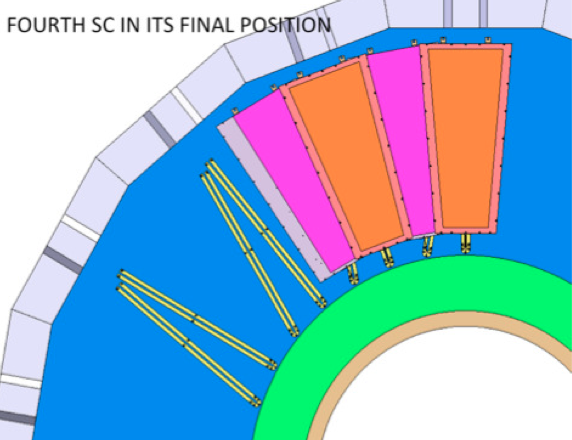
\includegraphics[height = 5.3cm]{gem/install_2.png}
                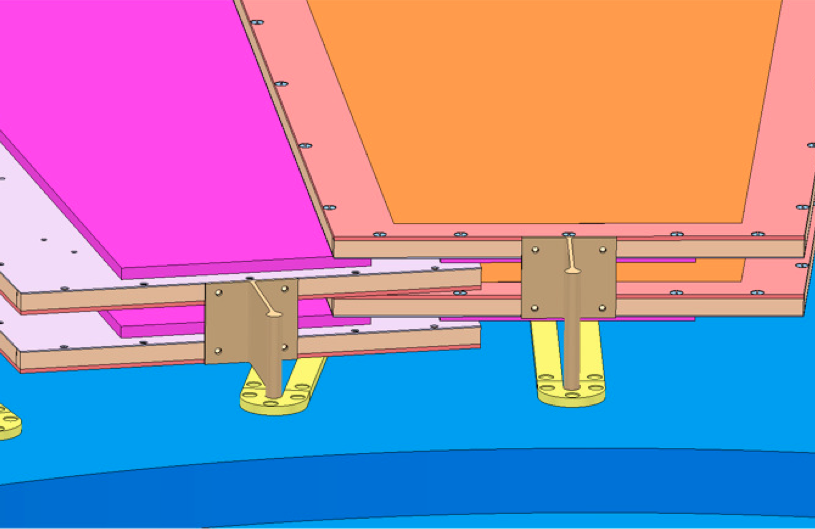
\includegraphics[height = 5.3cm]{gem/install_1.png}
                \caption{Disposition of the GEM prototypes on the yoke of CMS \Cite{GEM_Technical_Proposal}.}
                \label{fig:gas_electron_multiplier_detectors__install}
            \end{figure}    

        \subsection{Phase2 Installation}

            About Phase2

        \subsection{Phase3 Installation}

            About Phase3

    \section{Status of the GEM Project}

        Current status of the GEM project
